% Classe do documento e parâmetros gerais.
\documentclass[a4paper,openright,twoside,11pt]{report}

\usepackage[utf8]{inputenc}
\usepackage[english]{babel}
\addto{\captionsportuguese}{\renewcommand{\bibname}{Refer\^{e}ncias}}
\addto{\captionsportuguese}{\renewcommand{\contentsname}{\'{I}ndice}}

\usepackage{lipsum} % gerador de texto
\usepackage{graphicx}
\usepackage{url}
\usepackage[Algoritmo]{algorithm}
\usepackage{algorithmicx}
\usepackage{algpseudocode}
\renewcommand{\algorithmicrequire}{\textbf{Dados: }}
\renewcommand{\algorithmicensure}{\textbf{Resultado: }}

% pdflatex

% redefinição das margens das páginas
\setlength{\textheight}{24.00cm}
\setlength{\textwidth}{15.50cm}
\setlength{\topmargin}{0.35cm}
\setlength{\headheight}{0cm}
\setlength{\headsep}{0cm}
\setlength{\oddsidemargin}{0.25cm}
\setlength{\evensidemargin}{0.25cm}
\setlength{\textfloatsep}{16pt}


% Página inicial (capa)
\title{
   \vspace{-50mm}
   \begin{minipage}[l]{\textwidth}
      \hspace{-20mm}\resizebox{75mm}{!}{
\includegraphics{./figures/logoISELnew2.png}}\\
   \end{minipage}\\[20mm]
   {\huge \textbf{WaveCoach}\\[1ex]\LARGE Training Management Platform for Surf}
}

% Nome dos autores (um por linha)
\author{
\begin{tabular}{ll}
             & Tiago Canilhas  \\
             & João Barrisco \\[50mm]
\end{tabular}}

\date{
\begin{tabular}{ll}
  {Supervisores:} & Filipe Freitas \\
                  %& *Alberto Caeiro, SoftCompany*\\
\end{tabular}\\[10mm]
% Deixar o indicador respetivo em função da versão do relatório.
Relatório do projeto realizado no âmbito de Projecto e Seminário\\
Licenciatura em Engenharia Informática e de Computadores\\[20mm]
*Junho* de 2025}


\begin{document}
\pagenumbering{roman}
\thispagestyle{empty}
\maketitle

\baselineskip 18pt % line spacing: 12pt for single, 18pt for 1 1/2, and 24pt for double spacing

\newpage
\thispagestyle{empty}
% Fim da contracapa

% Página com identificação completa (número e nome) e assinaturas do(s) estudante(s) e do(s) orientador(es)
\cleardoublepage
\setcounter{page}{1}
\begin{center}
\textsc{\LARGE Instituto Superior de Engenharia de Lisboa}\\[50mm]

{\huge \textbf{WaveCoach}\\[1ex]\LARGE Training Management Platform for Surf}\\[20mm]

\begin{tabular}{rl}
  Tiago Canilhas, n.º50472, e-mail: a50472@alunos.isel.pt, tel.: 924115540\\[10mm]
           %& \rule{75mm}{0.5pt}\\[5mm]
  João Barrisco, n.º50476, e-mail: a50476@alunos.isel.pt, tel.: 967487235\\[10mm]
           %& \rule{75mm}{0.5pt}\\
\end{tabular}\\[10mm]

\begin{tabular}{rl}
  Supervisores: & Filipe Freitas, e-mail: ffreitas@cc.isel.ipl.pt \\[10mm]
               % & \rule{75mm}{0.5pt}\\[5mm]
               %  & *Alberto Joaquim Alves Caeiro, SoftCompany*\\[10mm]
               % & \rule{75mm}{0.5pt}\\
\end{tabular}\\[10mm]

Relatório do projeto realizado no âmbito de Projecto e Seminário\\
Licenciatura em Engenharia Informática e de Computadores\\[20mm]
*Junho* de 2025\\
\end{center}

% Página de resumo em Português
\cleardoublepage
\chapter*{Resumo}
Texto do resumo.
Breve descrição do projeto, dos resultados importantes e das conclusões: o objetivo é dar ao leitor uma visão global do projeto (não deve exceder uma página).

%{\bf Palavras-chave:} lista de palavras-chave separadas por ;.

%% Página de agradecimentos
%\cleardoublepage
%\chapter*{Agradecimentos}
%Texto dos agradecimentos. É opcional.\\

% Geração do índice de conteúdos
\cleardoublepage
\tableofcontents \cleardoublepage

% Geração do índice de figuras e de tabelas
%\listoffigures \cleardoublepage
%\listoftables \cleardoublepage

% Reiniciar a numeração de páginas
\setcounter{page}{1}
\pagenumbering{arabic}

% Capitulo 1
%
% Capítulo 1
%
\chapter{Introduction} \label{cap:introduction}

Este é o início do capítulo.

Exemplo de indentação do segundo parágrafo.

%
% Secção 1.1
%
\section{Introduction} \label{sec11}

The goal of this project is to develop a web application that allows the management of surfing athletes. This application is mainly aimed at coaches, but athletes can also access it to view their performance. Coaches will be able to register athletes, log different training sessions (e.g. gym, surf), record competition results, and monitor
performance through interactive charts. This will help them analyze progress and adjust training plans. This project is being developed to meet coaches' need for a more efficient and effective platform, replacing manual registration, which can be time-consuming and difficult to manage as the number of athletes grows. The platform not only saves time but also ensures greater accuracy and accessibility of data, allowing coaches to focus more on their athletes’ development and less on administrative tasks.


%
% Secção 1.2
%
\section{System Requirements} \label{sec12}

%
% Secção 1.2.1
%
\subsection{Functional Requirements} \label{sec121}
\begin{itemize}
\item \textbf{User registration:} Coaches should be able to register by providing a username and password.
\item \textbf{Athlete management:} Coaches should be able to add and remove their athletes. Adding an athlete will only require their name and date of birth.
\item \textbf{Athlete profile:} Coaches should be able to add and view information related to their athletes, such as weight, height, body mass index, and more. Athletes can also view this same information.
\item \textbf{Athletes' training records:} Coaches, through interactive tables and charts, should be able to record and track each athlete's training sessions. Each training session contains different information:
\begin{itemize}
\item \textbf{Surf training sessions:} Sea conditions, maneuvers performed, and a training-related questionnaire completed by the athlete.
\item \textbf{Gym training sessions:} Type of exercise, repetitions, and weight.
\end{itemize}
\item \textbf{Athletes' summaries:} The application should allow, weekly or monthly, summaries so that coaches and athletes can analyze the progress.
\item \textbf{Athletes' competition records:} Coaches can store data from their athletes' competitions, such as the date, location, and score achieved.
\end{itemize}
%
% Secção 1.2.2
%
\subsection{Non-Functional Requirements} \label{sec122}
\begin{itemize}
\item \textbf{User-friendly:} The application should be easy to understand, and therefore, it should have a simple and intuitive user interface.
\item \textbf{Cloud Deployment:} The application will be hosted on a cloud platform to ensure easy access. This will allow users to access the platform from anywhere without needing local installations.
\item \textbf{Tested:} The application must include tests to ensure that all functionalities work correctly.
\end{itemize}

%
% Secção 1.2.3
%
\subsection{Optional Features} \label{sec123}
\begin{itemize}
\item \textbf{PDF Generation:} The application should be able to generate a PDF file with the athlete's summaries, so the coach can interact with the summaries more easily.
\item \textbf{Planning of future training sessions:} In addition to accessing past training sessions, the coach will be able to schedule new training sessions by providing the date and type of training. Athletes will be able to access this information.
\item \textbf{Email notifications:} The application will notify athletes by email if any training session is scheduled or changed. For this, athletes will need to associate their email address.
\end{itemize}


%
% Secção 1.3
%
\section{Risks} \label{sec13}
\begin{itemize}
\item Having no knowledge of surfing practice may lead to difficulties in creating a practical design for coaches, as we don’t know the best way to present information to them. Consequently, frequent communication with the practitioners will be essential.
\item In frontend development, we may encounter more challenges because, although these technologies aren't new to us, we have less experience with TypeScript and React.
\end{itemize}

%
% Secção 1.4
%
\section{Plan} \label{sec14}
\begin{figure}[h]
\centering
\includegraphics [width=6in]{./figures/GanttChart.png}
\caption{Gantt Chart plan.}
\end{figure}

% Capitulo 2
%
% Capítulo 2
%
\chapter{Problem} \label{cap:Problem}

Este capítulo tem como objetivo explicar o contexto do projeto, ou seja demonstrar como é realizado o registo de treinos e competições, como é feita a gestão dos atletas e como é feito o planeamento do treino sem a utilização de uma plataforma digital.

\section{Workouts}

O principal registo realizado pelos treinadores é o registo dos treinos. Este registo é feito de forma manual, ou seja, o treinador tem de escrever num caderno ou numa folha de excel todos os treinos realizados pelos atletas. Este registo é feito para cada atleta individualmente e para cada treino realizado. O treinador tem de ter em conta a data do treino, o tipo de treino (se foi um treino de surf ou um treino de ginásio), os exercícios realizados ou as manobras realizadas.


\subsection{Gym workouts}

\subsection{Surf workouts}

\section{Mesocycles and microcycles}
\lipsum[3-5]



\section{Competitions}



% Capitulo 3
\chapter{Architecture} \label{cap:architecture}

A nossa solução é apresentada neste capítulo. A solução consiste em grandes ideias, desenvolvidas e testadas.

Exemplo de indentação do segundo parágrafo.

\section{Data model} \label{sec31}
Texto da secção. Seguem-se exemplos de vários parágrafos.

A avaliação de Projecto e Seminário envolve:
\begin{enumerate}
	\item proposta do projeto;
	\item relatório de progresso;
	\item apresentação individual;
	\item cartaz e versão beta do projeto;
	\item relatório de projeto e discussão pública final.
\end{enumerate}

A avaliação incide sobre o trabalho planeado e desenvolvido pelos estudantes, com constrições de tempo e prazos previamente estabelecidos. Se durante a realização do projeto for considerado que este está em risco, ouvidos os estudantes envolvidos, o orientador e o docente da unidade curricular decidem se o projeto continua. Em caso de desistência do estudante, esta deve ser comunicada ao orientador do projeto e ao regente da unidade curricular.

\section{Technologies} \label{sec32}
Na segunda secção deste capítulo, vamos abordar o enquadramento,
o contexto e as funcionalidades.


% Capitulo 4
\chapter{Backend} \label{cap:backend}

Este é o capítulo de testes. 
É possível forçar a inclusão de todas as referências com \cite{*}.

\section{Http}

\subsection{Interceptores}

\subsection{Controllers}

\section{Services}

\section{Repository}

\section{Data base}

% Capitulo 5
\chapter{Frontend} \label{cap:frontend}

A nossa solução é apresentada neste capítulo. A solução consiste em grandes ideias, desenvolvidas e testadas.

Exemplo de indentação do segundo parágrafo.

\section{Navegation} \label{sec51}
Texto da secção. Seguem-se exemplos de vários parágrafos.

\section{Components} \label{sec52}
Na segunda secção deste capítulo, vamos abordar o enquadramento,
o contexto e as funcionalidades.


% Capitulo 6
\chapter{Mobile App} \label{cap:mobileApp}

A nossa solução é apresentada neste capítulo. A solução consiste em grandes ideias, desenvolvidas e testadas.



% Capitulo 7
\chapter{Conclusion} \label{cap:conclusion}

A nossa solução é apresentada neste capítulo. A solução consiste em grandes ideias, desenvolvidas e testadas.


% Referências
\bibliographystyle{unsrt}
\bibliography{references}
\addcontentsline{toc}{chapter}{References}


\end{document} 

%\tableofcontents

%\newpage

%\section{Introduction}

%\subsection{Introduction}
%The goal of this project is to develop a web application that allows the management of surfing athletes. This application is mainly aimed at coaches, but athletes can also access it to view their performance. Coaches will be able to register athletes, log different training sessions (e.g. gym, surf), record competition results, and monitor
%performance through interactive charts. This will help them analyze progress and adjust training plans. This project is being developed to meet coaches' need for a more efficient and effective platform, replacing manual registration, which can be time-consuming and difficult to manage as the number of athletes grows. The platform not only saves time but also ensures greater accuracy and accessibility of data, allowing coaches to focus more on their athletes’ development and less on administrative tasks.

%\subsection{System Requirements}

%\subsubsection{Functional Requirements}
%\begin{itemize}
%\item \textbf{User registration:} Coaches should be able to register by providing a username and password.
%\item \textbf{Athlete management:} Coaches should be able to add and remove their athletes. Adding an athlete will only require their name and date of birth.
%\item \textbf{Athlete profile:} Coaches should be able to add and view information related to their athletes, such as weight, height, body mass index, and more. Athletes can also view this same information.
%\item \textbf{Athletes' training records:} Coaches, through interactive tables and charts, should be able to record and track each athlete's training sessions. Each training session contains different information:
%\begin{itemize}
%\item \textbf{Surf training sessions:} Sea conditions, maneuvers performed, and a training-related questionnaire completed by the athlete.
%\item \textbf{Gym training sessions:} Type of exercise, repetitions, and weight.
%\end{itemize}
%\item \textbf{Athletes' summaries:} The application should allow, weekly or monthly, summaries so that coaches and athletes can analyze the progress.
%\item \textbf{Athletes' competition records:} Coaches can store data from their athletes' competitions, such as the date, location, and score achieved.
%\end{itemize}

%\subsubsection{Non-Functional Requirements}
%\begin{itemize}
%\item \textbf{User-friendly:} The application should be easy to understand, and therefore, it should have a simple and intuitive user interface.
%\item \textbf{Cloud Deployment:} The application will be hosted on a cloud platform to ensure easy access. This will allow users to access the platform from anywhere without needing local installations.
%\item \textbf{Tested:} The application must include tests to ensure that all functionalities work correctly.
%\end{itemize}

%\subsubsection{Optional Features}
%\begin{itemize}
%\item \textbf{PDF Generation:} The application should be able to generate a PDF file with the athlete's summaries, so the coach can interact with the summaries more easily.
%\item \textbf{Planning of future training sessions:} In addition to accessing past training sessions, the coach will be able to schedule new training sessions by providing the date and type of training. Athletes will be able to access this information.
%\item \textbf{Email notifications:} The application will notify athletes by email if any training session is scheduled or changed. For this, athletes will need to associate their email address.
%\end{itemize}

%\subsection{Technologies}
%In the development of this project different technologies will be employed, such as the Kotlin programming language \cite{kotlin} and the Spring framework \cite{spring}, which will be utilized for the creation of the API. PostgreSQL \cite{postgresql} will also be used for data storage. Finally, TypeScript \cite{typescript} will be applied, together with the React library \cite{react}, for the creation of the website.

%\subsection{Risks}
%\begin{itemize}
%\item Having no knowledge of surfing practice may lead to difficulties in creating a practical design for coaches, as we don’t know the best way to present information to them. Consequently, frequent communication with the practitioners will be essential.
%\item In frontend development, we may encounter more challenges because, although these technologies aren't new to us, we have less experience with TypeScript and React.
%\end{itemize}

%\subsection{Plan}
%\begin{figure}[h]
%\centering
%\includegraphics [width=6in]{GanttChart.png}
%\caption{Gantt Chart plan.}
%\end{figure}

%\section{Problem}

%\section{Architecture}

%\section{Technologies}

%\section{Backend}

%\section{Frontend}

%\section{Conclusions}

%\bibliographystyle{unsrt}
%\bibliography{references}

%\end{document}